\section{Future Work}

An important problem which is actively being researched is the development of efficient extraction algorithms. Such algorithms are needed, because when we are done simplifying a circuit, we want to be able to extract a classical gate representation of the circuit in order to simulate it on real hardware. This generally is not a trivial task, since ZX-Diagrams are a superset of the classical quantum circuits\cite{duncan2020simplification} as seen in figure \ref{fig:extraction}.

\begin{figure}[h]
    \centering
    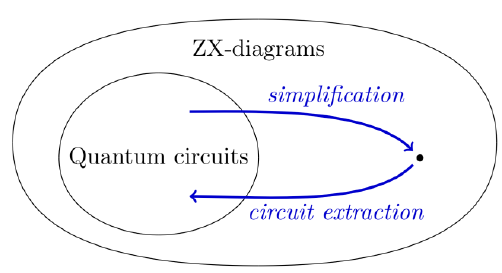
\includegraphics[width=0.35\textwidth]{images/extraction.png}
    \caption{Simplifcation process\cite{duncan2020simplification}}
    \label{fig:extraction}
\end{figure}